
\emph{Dans tout l'exercice, on n'attendait pas de justification, on en donne quelques unes dans ce corrigé quand même.}

\begin{enumerate}
\item Le bloc \begin{scratch} \blockmove{aller à x: \ovalnum{- 100} y: \ovalnum0} \end{scratch} indique que le lutin se positionne aux coordonnées $ (-100~;~0) $.

\item \begin{minipage}[t]{8.5cm}
	Voici la figure obtenue, en prenant 1 cm pour 20 pas :

	\medskip

	En effet, le script donne :
	\begin{itemize}[label=\textbullet]
		\item on place le lutin au point $ (-100,0) $;
		\item le lutin regarde vers la droite;
		\item la variable \og côté \fg{} prend la valeur 80;
		\item on avance de 80 pas (donc 4 cm, ici);
		\item le lutin tourne dans le sens  anti horaire de 120\degre, donc le prochain segment fera un angle de :

$ 180 - 120 = 60 $\degre avec le segment précédent;
		\item on recommence deux autres fois, en traçant des segments de 4 cm, formant un angle de 60\degre avec le segment précédent : on trace donc un triangle équilatéral de côté 4cm.

	\end{itemize}
\end{minipage}  \hfill
\begin{tikz}[baseline={(current bounding box.north)}]
	\draw (0,0)--(0:4cm)--(60:4cm)--(0,0)--(-60:4)--(0:4);
\end{tikz}
\begin{itemize}[label=\textbullet]
	\item après cette première boucle, on est donc revenu au point de départ (on a bouclé le triangle équilatéral) et on a tourné 3 fois de 120\degre, donc on a fait un tour complet ($3\times 120 = 360$\degre), on regarde donc dans le même sens qu'au début;
	\item la boucle suivante refait tracer un triangle équilatéral, avec le premier côté en commun, mais cette fois, on tourne dans l'autre sens.
\end{itemize}

\item Le script \no 1 trace le motif une première fois, se décale de 100 pas vers la droite (et donc est 20 pas à droite de la droite du motif précédent), trace à nouveau le motif, puis recommence une troisième fois : c'est la figure B.

Le script \no 2 trace le motif une première fois avec un côté de 80, puis, sans se déplacer, le trace une deuxième fois, avec un côté multiplié par 1,2 (soit 96 pas), puis une troisième fois avec un côté à nouveau multiplié par 1,2 (pour arriver à 115,2 pas de côté) : c'est la figure A.

Le script \no 3 est donc associé à la figure C, par élimination.

\begin{minipage}{10.5cm}
	On peut aussi le comprendre : on trace le motif une première fois, puis une deuxième fois, mais après avoir fait une rotation de 120\degre{} dont le centre est le point de départ, puis une troisième fois après une autre rotation.

On obtient la figure ci dessous, où le premier motif est en trait fin, le second en trait plus épais et le troisième encore plus épais :
\end{minipage}
\hfill
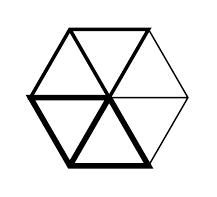
\begin{tikzpicture}[baseline={(0,0)}]
	\draw[line width=0.5pt] (0,0)--(-60:1)--(0:1)--(60:1)--cycle--(0:1);
	\draw[line width=1.25pt] (0,0)--(60:1)--(120:1)--(180:1)--cycle--(120:1);
	\draw[line width=2pt] (0,0)--(180:1)--(240:1)--(300:1)--cycle--(240:1);
	content
\end{tikzpicture}
\item Dans cette question on s'intéresse au script \no 2.
	\begin{enumerate}
		\item Le bloc \og motif \fg{} est exécuté trois fois.
		\item À la fin de ce script, la variable côté a été multipliée trois fois par 1,2 donc sa valeur est : \quad $80 \times 1,2^3 = 138,24$.

Cependant, aucun motif n'est tracé avec ce côté là, s'il y avait 4 répétitions, le quatrième motif serait tracé avec un côté de 138,24 pas, et la variable terminerait à la valeur $80\times 1,2^4$.
	\end{enumerate}
\end{enumerate}
